\documentclass[pdflatex,compress,mathserif]{beamer}

%\usetheme[dark,framenumber,totalframenumber]{ElektroITK}
\usetheme[darktitle,framenumber,totalframenumber]{ElektroITK}

\usepackage{amsmath}
\usepackage{graphicx}
\usepackage{multicol}
\usepackage[bahasai]{babel}

\newcommand*{\Scale}[2][4]{\scalebox{#1}{$#2$}}%

\title{METODE NUMERIK}
\subtitle{Solusi Sistem Persamaan Lanjar}

\author{Tim Dosen Pengampu}

\begin{document}
	
\maketitle

\section{Pengantar}

\begin{frame}
	\frametitle{Pengantar}
	\begin{itemize}
		\item \textbf{Persoalan:} Temukan vektor x yang memenuhi sistem persamaan lanjar \[ Ax = b \] yang dalam hal ini,
		\begin{align*}
			A &= [a_{ij}] \text{ adalah matriks berukuran } n \times n\\
			x &= [x_{j}]  \text{ adalah matriks berukuran } n \times n1 \\
			b &= [b_{j}]  \text{ adalah matriks berukuran } n \times 1 \text{ (vektor kolom) }
		\end{align*}
	\end{itemize}
\end{frame}

\begin{frame}[t]
	\[
	\begin{matrix}
	a_{11}x_1 + a_{12}x_2 + \dots + a_{1n}x_n &= b_1 \\
	a_{21}x_1 + a_{22}x_2 + \dots + a_{2n}x_n &= b_2 \\
	&\vdots\\
	a_{n1}x_1 + a_{n2}x_2 + \dots + a_{nn}x_n &= b_n
	\end{matrix}
	\]
	\[\downarrow\]
	\[
	\begin{bmatrix}
		a_{11} & a_{12} & a_{13} & \dots & a_{1n} \\
		a_{21} & a_{22} & a_{23} & \dots & a_{2n} \\
		a_{31} & a_{32} & a_{33} & \dots & a_{3n} \\
		& & & \vdots &  \\
		a_{n1} & a_{n2} & a_{n3} & \dots & a_{nn}
	\end{bmatrix}
	\begin{bmatrix}
		x_1 \\
		x_2 \\
		x_3 \\
		\vdots\\
		x_n \\
	\end{bmatrix}
	=
	\begin{bmatrix}
		b_1 \\
		b_2 \\
		b_3 \\
		\vdots\\
		b_n \\
	\end{bmatrix}
	\]
\end{frame}

\begin{frame}
	\frametitle{Metode-Metode Penyelesaian}
	\begin{itemize}
		\item Metode penyelesaian praktis sistem persamaan lanjar yang dibahas di sini adalah:
		\begin{enumerate}
			\item Metode eliminasi Gauss 
			\item Metode eliminasi Gauss-Jordan
			\item Metode matriks balikan
			\item Metode dekomposisi LU
			\item Metode lelaran Jacobi
			\item Metode lelaran Gauss-Seidel.
		\end{enumerate}
		\item Metode 2, 3, da, 4, didasarkan pada Metode 1
		\item Metode 5 dan 6 dikembangkan dari gagasan metode lelaran pada solusi persamaan nirlanjar
	\end{itemize}
\end{frame}

\section{Metode Eliminasi Gauss}

\begin{frame}
	\frametitle{Metode Eliminasi Gauss}
	\begin{itemize}
		\item Metode ini berangkat dari kenyataan bahwa bila matriks A berbentuk segitiga atas seperti sistem persamaan berikut ini
		\begin{equation*}
			\begin{bmatrix}
				a_{11} & a_{12} & a_{13} & \cdots & a_{1n}\\
				0 & a_{22} & a_{23} & \cdots & a_{2n}\\
				0 & 0 & a_{e3} & \cdots & a_{en}\\
				& & & \vdots & \\
				0 & 0 & 0 & \cdots & a_{nn}\\
			\end{bmatrix}
			\begin{bmatrix}
			x_1\\
			x_2\\
			x_3\\
			\vdots\\
			x_n\\
			\end{bmatrix}
			=
			\begin{bmatrix}
			b_1\\
			b_2\\
			b_3\\
			\vdots\\
			b_n\\
			\end{bmatrix}
		\end{equation*}
		\item maka solusinya dapat dihitung dengan \textbf{teknik penyulihan
		mundur} (backward substitution)
	\end{itemize}
\end{frame}

\begin{frame}
	\begin{itemize}
		\item[] $ a_{nn}x_n = b_n \rightarrow x_n = b_n / a_{nn} $
		\item[] $ a_{n-1,n-1}x_{n-1} + a_{n-1,n}x_{n} = b_{n-1} \rightarrow x_{n-1} = \frac{b_{n-1} - a_{n-1,n}x_n}{a_{n-1,n-1}}$
		\item[] $ a_{n-2,n-2}x_{n-2} + a_{n-2,n-1}x_{n-1} + a_{n-2,n}x_{n} = b_{n-2} \rightarrow x_{n-2} = \frac{b_{n-2} - a_{n-2,n-1}x_{n-1} - a_{n-2,n}x_{n}}{a_{n-2,n-2}}$
		\item[] $\dots$ dst
		\item Sekali $ x_n $, $ x_{n-1} $, $ x_{n-2} $, $\dots$, $ x_{k+1} $ diketahui, maka nilai $ x_k $ dapat dihitung dengan
		\[ x_k = \frac{b_k - \sum_{j=k+1}^{n}a_{kj}x_j}{a_{kk}}.\qquad k=n-1, n-2, \dots, 1 \text{ dan } a_{kk} \neq 0 \]
	\end{itemize}
\end{frame}

\begin{frame}
	\frametitle{Contoh 1}
	\begin{itemize}
		\item Selesaikan sistem persamaan lanjar berikut dengan teknik penyulihan mundur
		\begin{align*}
			4x_1 - x_2 + 2x_3 + 3x_4 &= 20 \\
			-2x_2 + 7x_3 - 4x_4 &= -7 \\
			6x_3 + 5x_4 &= 4 \\
			3x_4 &= 6
		\end{align*}
	\end{itemize}
\end{frame}

\begin{frame}
	\begin{itemize}
		\item Penyelesaian:
		\begin{align*}
		x_4 &= 6/3 = 2 \\
		x_3 &= \frac{(4-5(2))}{6} = -1 \\
		x_2 &= \frac{-7-7(-1)+4(2)}{-2} = -4 \\
		x_1 &= \frac{20 + 1(-4) - 2(-1)-3(2)}{4} = 3
		\end{align*}
		\item Jadi, solusinya adalah \[ x = \begin{bmatrix}
			3 \\ -4 \\ -1 \\ 2
		\end{bmatrix} \]
	\end{itemize}
\end{frame}

\begin{frame}
	\begin{itemize}
		\item Metode eliminasi Gauss pada prinsipnya bertujuan mentransformasi sistem $ Ax = b $ menjadi sistem \[ Ux = y \] dengan $ U $ adalah matriks segitiga atas. Selanjutnya solusi $ x $ dapat dihitung dengan teknik penyulihan mundur
	\end{itemize}
\end{frame}

\begin{frame}
	\begin{align*}
	[A,b]
	&\rightarrow
	[U,y]
	\\
	\left[
	\begin{matrix}
	a_{11} & a_{12} & a_{13} & a_{14}\\
	a_{21} & a_{22} & a_{23} & a_{24}\\
	a_{31} & a_{32} & a_{33} & a_{34}\\
	a_{41} & a_{42} & a_{43} & a_{44}
	\end{matrix}
	\right|
	\left.
	\begin{matrix}
	b_{1}\\
	b_{2}\\
	b_{3}\\
	b_{4}
	\end{matrix}
	\right]
	&\rightarrow
	\left[
	\begin{matrix}
	a_{11} & a_{12} & a_{13} & a_{14}\\
	0 & a_{22}^{(1)} & a_{23}^{(1)} & a_{24}^{(1)}\\
	0 & 0 & a_{33}^{(2)} & a_{34}^{(2)}\\
	0 & 0 & 0 & a_{44}^{(3)}
	\end{matrix}
	\right|
	\left.
	\begin{matrix}
	b_{1}\\
	b_{2}^{(1)}\\
	b_{3}^{(2)}\\
	b_{4}^{(3)}
	\end{matrix}
	\right]
	\end{align*}
\end{frame}

\begin{frame}
	Proses eliminasi terdiri atas tiga operasi baris elementer:
	\begin{enumerate}
		\item Pertukaran : Urutan dua persamaan dapat ditukar karena pertukaran tersebut tidak mempengaruhi solusi akhir.
		\item Penskalaan : Persamaan dapat dikali dengan konstanta bukan nol, karena perkalian tersebut tidak mempengaruhi solusi akhir.
		\item Penggantian : Persamaan dapat diganti dengan penjumlahan persamaan itu dengan gandaan persamaan lain. Misalnya persamaan diganti dengan selisih persamaan itu dengan dua kali persamaan lain; yaitu
		\[ \text{baris}_r := \text{baris}_r - m_{p,r}\text{baris}_p \]
	\end{enumerate}
\end{frame}

\begin{frame}
	\begin{itemize}
		\item Nilai $ a_{r, r} $ pada posisi $ (r, r) $ yang digunakan untuk mengeliminasi $ x_r $ pada baris $ r + 1, r + 2, \dots, N $ dinamakan \textbf{elemen pivot} dan persamaan pada baris ke-$ r $ disebut \textbf{persamaan pivot}.
		\item Ada kemungkinan pivot bernilai nol sehingga pembagian dengan nol tidak dapat dielakkan.
		\item Tata-ancang eliminasi yang tidak mempedulikan nilai pivot adalah tatancang yang naif (naive) atau sederhana. Metode eliminasi Gauss seperti ini dinamakan \textbf{metode eliminasi Gauss naif} (\textit{naive Gaussian elimination}).
		\item Pada metode eliminasi Gauss naif tidak ada operasi pertukaran baris dalam rangka menghindari pivot yang bernilai nol itu.
	\end{itemize}
\end{frame}

\begin{frame}
	\frametitle{Contoh 2}
	\begin{itemize}
		\item Selesaikan sistem persamaan lanjar dengan metode eliminasi Gauss naif:
		\begin{align*}
			2x_1 + 3x_2 - x_3 &= 5 \\
			4x_1 + 4x_2 - 3x_3 &= 3 \\
			-2x_1 + 3x_2 - x_3 &= 1
		\end{align*}
	\end{itemize}
\end{frame}

\begin{frame}
	\begin{itemize}
		\item Penyelesaian
	\end{itemize}
	\begin{align*}
	\Scale[0.8]{
		\left[
		\begin{matrix}
		\textbf{2} & 3 & -1 \\
		4 & 4 & -3 \\
		-2 & 3 & -1
		\end{matrix}
		\right|
		\left.
		\begin{matrix}
		5 \\
		3 \\
		1
		\end{matrix}
		\right]
		\begin{matrix}
		 \\
		R_2 - \frac{4}{2}R_1 \\
		R_3 - \frac{-2}{2}R_1
		\end{matrix}
		\left[
		\begin{matrix}
		2 & 3 & -1 \\
		0 & \textbf{-2} & -1 \\
		0 & 6 & -2
		\end{matrix}
		\right|
		\left.
		\begin{matrix}
		5 \\
		-7 \\
		6
		\end{matrix}
		\right]
		\begin{matrix}
		\\
		\\
		R_3 - \frac{6}{-2}R_1
		\end{matrix}
		\left[
		\begin{matrix}
		2 & 3 & -1 \\
		0 & -2 & -1 \\
		0 & 0 & -5
		\end{matrix}
		\right|
		\left.
		\begin{matrix}
		5 \\
		-7 \\
		-15
		\end{matrix}
		\right]}
	\end{align*}
\end{frame}

\begin{frame}
	\begin{itemize}
		\item Solusi sistem diperoleh dengan teknik penyulihan mundur sebagai berikut:
		\begin{align*}
			-5x_3 = -15 &\rightarrow x_3 = 3 \\
			-2x_2 - x_3 = -7 &\rightarrow x_2 = (-7 + 3)/-2 = 2 \\
			2x_1 + 3x_2 - x_3 = 5 &\rightarrow x_1 = (5 + 3 - 6)/2 = 1
		\end{align*}
		\item Jadi, solusinya adalah \[ x = 
		\begin{bmatrix}
		1 \\ 2 \\ 3 
		\end{bmatrix} \]
	\end{itemize}
\end{frame}

\begin{frame}
	\frametitle{Kelemahan eliminasi Gauss naif}
	\begin{itemize}
		\item Jika pivot $ a_{pp} = 0 $, baris ke-$ k $ tidak dapat digunakan untuk memgeliminasi elemen pada kolom $ p $, karena terjadinya pembagian dengan nol.
		\item Oleh karena itu, pivot yang bernilai nol harus dihindari dengan tata-ancang (\textit{strategy}) pivoting.
	\end{itemize}
\end{frame}

\subsection{Tata-ancang Pivoting}

\begin{frame}
	\frametitle{Tata-ancang Pivoting}
	\begin{itemize}
		\item jika $ a_{p,p}^{(p-1)} = 0 $, cari baris $ k $ dengan $ a_{k,p} \neq 0 $ dan $ k > p $, lalu pertukarkan baris $ p $ dan baris $ k $.
		\item Metode eliminasi Gauss dengan tata-ancang pivoting disebut metode eliminasi Gauss yang diperbaiki (\textit{modified Gaussian elimination}).
	\end{itemize}
\end{frame}

\begin{frame}
	\frametitle{Contoh 3}
	\begin{itemize}
		\item Selesaikan sistem persamaam lanjar berikut dengan metode eliminasi Gauss yang menerapkan tatancang pivoting.
		\begin{align*}
			x_1 + 2x_2 + x_3 &= 2 \\
			3x_1 + 6x_2 &= 9 \\
			2x_1 + 8x_2 + 4x_3 &= 6
		\end{align*}
	\end{itemize}
\end{frame}

\begin{frame}
	\begin{itemize}
		\item Penyelesaian
	\end{itemize}
	
	\[
	\left[
		\begin{matrix}
			\textbf{1} & 2 & 1 \\
			3 & 6 & 0 \\
			2 & 8 & 4
		\end{matrix}
	\right|
	\left.
		\begin{matrix}
			2 \\
			9 \\
			6
		\end{matrix}
	\right]
	\begin{matrix}
		\\
		R_2 - \frac{3}{1}R_1 \\
		R_3 - \frac{2}{1}R_1
	\end{matrix}
	\left[
		\begin{matrix}
			1 & 2 & 1 \\
			0 & \textbf{0} & -3 \\
			0 & 4 & 2
		\end{matrix}
	\right|
	\left.
		\begin{matrix}
			2 \\
			3 \\
			2
		\end{matrix}
	\right]
	\begin{matrix}
	\\
	R_2 \Leftrightarrow R_3\\
	\end{matrix}
	\left[
	\begin{matrix}
	1 & 2 & 1 \\
	0 & 4 & 2 \\
	0 & 0 & -3
	\end{matrix}
	\right|
	\left.
	\begin{matrix}
	2 \\
	2 \\
	3
	\end{matrix}
	\right]
	\]
\end{frame}

\begin{frame}
	\frametitle{Pivoting Sederhana}
	\begin{itemize}
		\item Melakukan pertukarkan baris untuk menghindari pivot yang bernilai nol adalah cara pivoting yang sederhana (simple pivoting).
		\item Masalah lain dapat juga timbul bila elemen pivot sangat dekat ke nol, karena jika elemen pivot sangat kecil dibandingkan terhadap elemen lainnya, maka galat pembulatan dapat muncul.
		\item Jadi, disamping menghindari pembagian dengan nol, tatancang pivoting dapat juga diperluas untuk mengurangi galat pembulatan.
		\item Terdapat 2 macam pivoting yaitu pivoting sebagian dan pivoting lengkap.
	\end{itemize}
\end{frame}

\begin{frame}
	\frametitle{Pivoting Sebagian}
	\begin{itemize}
		\item Pada tatancang pivoting sebagian, pivot dipilih dari semua elemen pada kolom $ p $ yang mempunyai nilai mutlak terbesar,
		\[ |a_{k,p}| = \text{max}\{|a_{p,p}|,|a_{p+1,p}|,\dots,|a_{n-1,p}|, |a_{n,p}|\} \]
		\item  lalu pertukarkan baris ke-$ k $ dengan baris ke-$ p $.
		\[
		\left[
		\begin{matrix}
			x & x & x & x \\
			0 & \textbf{x} & x & x \\
			0 & \textbf{x} & x & x \\
			0 & \textbf{x} & x & x \\
		\end{matrix}
		\right|
		\left.
		\begin{matrix}
		x \\ x \\ x \\ x
		\end{matrix}
		\right]
		\] cari $ |\textbf{x}| $ terbesar, lalu pertukarkan barisnya dengan baris ke-2
	\end{itemize}
\end{frame}

\begin{frame}
	\begin{itemize}
		\item Perhatikanlah bahwa teknik pivoting sebagian juga sekaligus menghindari pemilihan pivot = 0 (sebagaimana pada simple pivoting)
		\item karena 0 tidak akan pernah menjadi elemen dengan nilai mutlak terbesar, kecuali jika seluruh elemen di kolom yang diacu adalah 0.
		\item Apabila setelah melakukan pivoting sebagian ternyata elemen pivot = 0, itu berarti sistem persamaan lanjar tidak dapat diselesaikan (singular system).
	\end{itemize}
\end{frame}

\begin{frame}
	\frametitle{Pivoting Lengkap}
	\begin{itemize}
		\item Jika disamping baris, kolom juga diikutkan dalam pencarian elemen terbesar dan kemudian dipertukarkan, maka tata ancang ini disebut pivoting lengkap.
		\item Pivoting lengkap jarang dipakai dalam program sederhana karena pertukaran kolom mengubah urutan suku $ x $ dan akibatnya menambah kerumitan program secara berarti.
	\end{itemize}
\end{frame}

\begin{frame}
	\frametitle{Contoh 4}
	\begin{itemize}
		\item Dengan menggunakan empat angka bena, selesaikan sistem persamaan berikut dengan metode eliminasi Gauss:
		\begin{align*}
			0.0003x_1 + 1.566x_2 &= 1.569 \\
			0.3454x_1 - 2.436x_2 &= 1.018
		\end{align*}
		\begin{enumerate}
			\item tanpa tata ancang pivoting sebagian (Gauss naif)
			\item dengan tata ancang pivoting sebagian (Gauss yang dimodifikasi)
		\end{enumerate}
		\item (Perhatikan, dengan 4 angka bena, solusi sejatinya adalah $ x_1 = 10.00 $ dan $ x_2 = 1.00 $)
	\end{itemize}
\end{frame}

\begin{frame}
	\begin{itemize}
		\item Penyelesaian:
		\begin{enumerate}
			\item tanpa tata ancang pivoting sebagian (Gauss naif)
			\[
			\left[
				\begin{matrix}
				\textbf{0.0003} & 1.566 \\
				0.3454 & -2.436
				\end{matrix}
			\right|			
			\left.
			\begin{matrix}
				1.569 \\ 1.018
			\end{matrix}
			\right]
			\]
			Operasi baris pertama (0.0003 sebagai pivot):
			\[ R_2 \leftarrow R_2 - \frac{0.3454 R_1}{0.0003} = R_2 - 1151R_1\]
			(tanda “$\leftarrow$” berarti “diisi” atau “diganti dengan”)
		\end{enumerate}
	\end{itemize}
\end{frame}

\begin{frame}
	\begin{itemize}
		\item[]
		\begin{enumerate}
			\item[] Jadi,
			\begin{align*}
				a_{21} &\approx 0 \\
				a_{22} &\approx -2.436 - (1151)(1.566) \approx -2.436 - 1802 \approx -1804 \\
				b_2 &\approx 1.018 - (1151)(1.569) \approx 1.018 - 1806 \approx -1805
			\end{align*}
			\[
			\left[
				\begin{matrix}
					0.0003 & 1.566 \\
					0.3454 & -2.436
				\end{matrix}
			\right|
			\left.
				\begin{matrix}
					1.569 \\ 1.018
				\end{matrix}
			\right]
			\begin{matrix}
				\\
				R_2 -1151R_1
			\end{matrix}
			\left[
				\begin{matrix}
					0.0003 & 1.566 \\
					0 & -1804
				\end{matrix}
			\right|
			\left.
				\begin{matrix}
					1.569 \\ -1805
				\end{matrix}
			\right]
			\]
			Solusinya diperoleh dengan teknik penyulihan mundur:
			\begin{align*}
				x_2 &= -1805/-1804 = 1.001 \\
				x_2 &= \frac{1.569 - ( 1.566 )( 1.001 )}{0.0003} = \frac{1.569 - 1.568}{0.0003} = \frac{0.001}{0.0003} = 3.333
			\end{align*}
			(jauh dari solusi sejati)
		\end{enumerate}
	\end{itemize}
\end{frame}

\begin{frame}
	\begin{itemize}
		\item Jadi, $ x = (3.333, 1.001)^T $.
		\item Solusi ini sangat jauh berbeda dengan solusi sejatinya.
		\item Kegagalan ini terjadi karena $ | a_{11} | $ sangat kecil dibandingkan $ |x_{12} | $, sehingga galat pembulatan yang kecil pada $ x_2 $ menghasilkan galat besar di $ x_1 $ .
		\item Perhatikan juga bahwa $ 1.569 - 1.568 $ adalah pengurangan dua buah bilangan yang hampir sama, yang menimbulkan hilangnya angka bena pada hasil pengurangannya (loss of significance).
	\end{itemize}
\end{frame}

\begin{frame}
	\begin{itemize}
		\item Penyelesaian:
		\begin{enumerate}
			\item Baris pertama dipertukarkan dengan baris kedua sehingga 0.3454 menjadi pivot
			\[
			\left[
				\begin{matrix}
					\textbf{0.3454} & -2.436 \\
					0.0003 & 1.566 \\
				\end{matrix}
			\right|			
			\left.
				\begin{matrix}
					1.018 \\ 1.569 
				\end{matrix}
			\right]
			\begin{matrix}
				\\
				R_2 - \frac{0.0003}{0.3454}R_1
			\end{matrix}
			\left[
				\begin{matrix}
					0.3454 & -2.436 \\
					0 & 1.568 \\
				\end{matrix}
			\right|			
			\left.
				\begin{matrix}
					1.018 \\ 1.568 
				\end{matrix}
			\right]
			\]
			Dengan teknik penyulihan mundur diperoleh
			\begin{align*}
				x_2 &= 1.568 / 1.568 = 1.000 \\
				x_1 &= \frac{1.018-(-2.436)(1.000)}{0 . 3454} = 10.02
			\end{align*}
			\item[] Jadi, solusinya adalah $ x = (10.02, 1.000)^T $ , yang lebih baik daripada solusi sebelumnya.
		\end{enumerate}
	\end{itemize}
\end{frame}

\begin{frame}
	\begin{itemize}
		\item[]
		\begin{enumerate}
			\item[] Keberhasilan ini karena $ | a_{21} | $ tidak sangat kecil dibandingkan dengan $ | a_{22} | $, sehingga galat pembulatan yang kecil pada $ x_2 $ tidak akan menghasilkan galat yang besar pada $ x_1 $ .
		\end{enumerate}
	\end{itemize}
\end{frame}

\subsection{Kemungkinan Solusi SPL}

\begin{frame}
	\frametitle{Kemungkinan Solusi SPL}
	\begin{itemize}
		\item Tidak semua SPL mempunyai solusi. Ada tiga kemungkinan solusi yang dapat terjadi pada SPL:
		\begin{enumerate}
			\item mempunyai solusi yang unik,
			\item mempunyai banyak solusi, atau
			\item tidak ada solusi sama sekali.
		\end{enumerate}
	\end{itemize}
	\begin{center}
		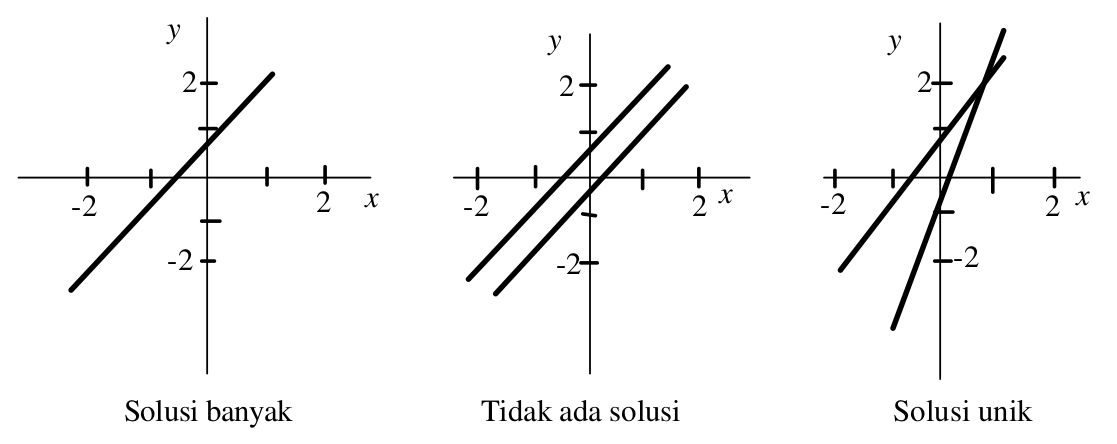
\includegraphics[width=0.9\linewidth]{img/img01}
	\end{center}
\end{frame}

\begin{frame}
	\begin{itemize}
		\item Untuk SPL dengan tiga buah persamaan atau lebih (dengan tiga peubah atau lebih), tidak terdapat tafsiran geometrinya seperti pada SPL dengan dua buah persamaan.
		\item Namun, kita masih dapat memeriksa masing-masing kemungkinan solusi itu berdasarkan pada bentuk matriks akhirnya.
	\end{itemize}
\end{frame}

\begin{frame}
	\frametitle{Solusi unik/tunggal}
	\[
	\left[
		\begin{matrix}
			1 & 1 & 1\\
			2 & 3 & 1\\
			3 & 1 & 2\\
		\end{matrix}
	\right|
	\left.
		\begin{matrix}
			0 \\ 1 \\ 1
		\end{matrix}
	\right]
	\xrightarrow{\text{Eliminasi Gauss}}
	\left[
		\begin{matrix}
			1 & 1 & 1\\
			0 & 1 & -1\\
			0 & 0 & -3\\
		\end{matrix}
	\right|
	\left.
		\begin{matrix}
			0 \\ 1 \\ 3
		\end{matrix}
	\right]
	\]
	Solusi: $ x_1 = 1 $, $ x_2 = 0 $, $ x_3 = -1 $
\end{frame}

\begin{frame}
	\frametitle{Solusi banyak/tidak terhingga}
	\[
	\Scale[0.8]{
	\left[
	\begin{matrix}
	1 & 1 & 2\\
	2 & -1 & 1\\
	1 & 2 & 3\\
	\end{matrix}
	\right|
	\left.
	\begin{matrix}
	4 \\ 2 \\ 6
	\end{matrix}
	\right]
	\xrightarrow{\text{Eliminasi Gauss}}
	\left[
	\begin{matrix}
	1 & 1 & 2\\
	0 & -3 & -3\\
	0 & 0 & 0\\
	\end{matrix}
	\right|
	\left.
	\begin{matrix}
	4 \\ -6 \\ 0
	\end{matrix}
	\right]
	}\]
	\begin{itemize}
		\item Perhatikan hasil eliminasi Gauss pada baris terakhir. Persamaan yang bersesuaian dengan baris terakhir tersebut adalah
		\[ 0x_1 + 0x_2 + 0x_3 = 0 \]
		yang dipenuhi oleh banyak nilai x.
		\item Solusinya diberikan dalam bentuk parameter:
		\item Misalkan $ x_3 = k $ maka $ x_2 = -6 + 3k $ dan $ x_1 = 10-5k $, dengan $ k \in R $
		\item Terdapat tidak berhingga nilai k, berarti solusi SPL banyak sekali.
	\end{itemize}
\end{frame}

\begin{frame}
	\frametitle{Tidak ada solusi}
	\[
	\Scale[0.8]{
		\left[
		\begin{matrix}
		1 & 1 & 2\\
		2 & -1 & 1\\
		1 & 2 & 3\\
		\end{matrix}
		\right|
		\left.
		\begin{matrix}
		4 \\ 2 \\ 7
		\end{matrix}
		\right]
		\xrightarrow{\text{Eliminasi Gauss}}
		\left[
		\begin{matrix}
		1 & 1 & 2\\
		0 & -3 & -3\\
		0 & 0 & 0\\
		\end{matrix}
		\right|
		\left.
		\begin{matrix}
		4 \\ -6 \\ 0
		\end{matrix}
		\right]
	}\]
	\begin{itemize}
		\item Perhatikan hasil eliminasi Gauss pada baris terakhir. Persamaan yang bersesuaian dengan baris terakhir tersebut adalah
		\[ 0x_1 + 0x_2 + 0x_3 = 1 \]
		yang dalam hal ini, tidak nilai $ x_i $ yang memenuhi, $ i = 1, 2, 3 $
	\end{itemize}
\end{frame}

\begin{frame}
	\begin{itemize}
		\item Bentuk akhir matriks setelah eliminasi Gauss untuk ketiga kemungkinan solusi di atas dapat digambarkan sebagai berikut:
	\end{itemize}
	\begin{center}
		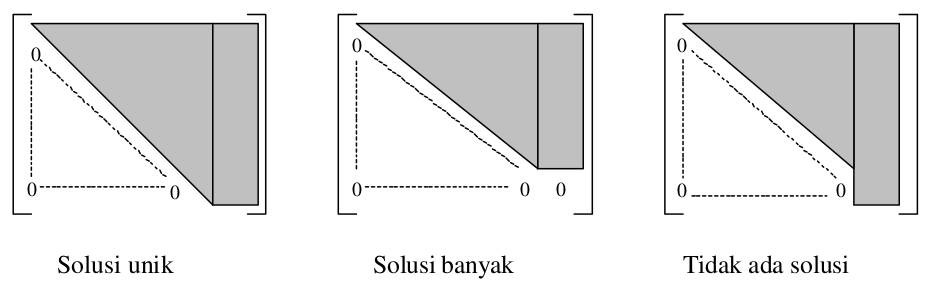
\includegraphics[width=0.9\linewidth]{img/img02}
	\end{center}
\end{frame}

\begin{frame}
	\begin{itemize}
		\item Kita rangkum “pertanda” kemungkinan solusi SPL di bawah ini:
		\begin{enumerate}
			\item Jika pada hasil eliminasi Gauss tidak terdapat baris yang semuanya bernilai 0 (termasuk elemen pada baris yang bersesuaian pada vektor kolom $ b $), maka solusi SPL dipastikan unik.
			\item Jika pada hasil eliminasi Gauss terdapat paling sedikit satu baris yang semuanya bernilai 0 (termasuk elemen pada baris yang bersesuaian pada vektor kolom $ b $), maka SPL mempunyai banyak solusi.
			\item Jika pada hasil eliminasi Gauss terdapat baris yang semuanya bernilai 0 tetapi elemen pada baris yang bersesuaian pada vektor kolom $ b $ tidak 0, maka SPL tidak mempunyai solusi.
		\end{enumerate}
	\end{itemize}
\end{frame}

\section{Metoda Eliminasi Gauss-Jordan}

\begin{frame}
	\frametitle{Metoda Eliminasi Gauss-Jordan}
	\begin{itemize}
		\item Metode eliminasi Gauss-Jordan merupakan variasi dari metode eliminasi Gauss.
		\item Dalam hal ini, matriks $ A $ dieliminasi menjadi matriks identitas $ I $.
		\[ Ax = b \rightarrow Ix = b' \]
		\item Tidak diperlukan lagi teknik penyulihan mundur untuk memperoleh solusi SPL. Solusinya langsung diperoleh dari vektor kolom $ b $ hasil proses eliminasi.
	\end{itemize}
\end{frame}

\begin{frame}
	\frametitle{Contoh 5}
	\begin{itemize}
		\item Selesaikan sistem persamaan lanjar di bawah ini dengan metode eliminasi Gauss-Jordan.
		\begin{align*}
		3x_1 - 0.1x_2 - 0.2x_3 = 7.85 \\
		0.1x_1 + 7x_2 - 0.3x_3 = -19.3 \\
		0.3x_1 - 0.2x_2 + 10x_3 = 71.4
		\end{align*}
	\end{itemize}
\end{frame}

\begin{frame}
	\begin{itemize}
		\item Penyelesaian:
	\end{itemize}
	\[
	\left[
		\begin{matrix}
			3 & -0.1 & -0.2 \\
			0.1 & 7 & -0.3 \\
			0.3 & -0.2 & 10
		\end{matrix}
	\right|
	\left.
		\begin{matrix}
			7.85 \\ -19.3 \\ 71.4
		\end{matrix}
	\right]
	\]
\end{frame}



\end{document}